\documentclass{article}

\usepackage{amsmath, amsthm, mathtools}
\usepackage{thmtools}

\newcommand{\HRule}[1]{\rule{\linewidth}{#1}}

\declaretheoremstyle[name=Theorem,]{thmsty}
\declaretheorem[style=thmsty,numberwithin=section]{theorem}

\declaretheoremstyle[name=Definition,]{prosty}
\declaretheorem[style=prosty,numberlike=theorem]{definition}

\newtheorem{lemma}{Lemma}[section]

\newcommand*{\successor}{%
    \stackrel{\scriptscriptstyle\!+\!}\longrightarrow%
}

\newcommand*{\lsuccessor}{%
    \stackrel{\scriptscriptstyle\!+\!}\longleftarrow%
}

\newcommand*{\too}{%
    \stackrel{\scriptscriptstyle\!*\!}\longrightarrow%
}

\newcommand*{\ltoo}{%
    \stackrel{\scriptscriptstyle\!*\!}\longleftarrow%
}

\begin{document}

\title{Lecture Notes}
\maketitle
\newpage

\tableofcontents
\newpage


\section{Lecture 3}

\subsection{Properties of abstract reduction systems}

In this lecture, we explore some properties of abstract reduction systems and look at the relationships between them.

\begin{definition}
    An abstract reduction system $( A, \xrightarrow[A]{} )$ is said to be \textbf{Church-Rosser} if $$\forall x, y \in A, \quad x \xleftrightarrow[A]{*} y \implies x \downarrow_A y$$
\end{definition}

Consider abstract reduction systems $A$ and $B$ as shown in the figure below. System $A$ is not Church-Rosser, since $a \xleftrightarrow[A]{*} b$ but $a$ and $b$ are not joinable. System $B$ is a simple example of a Church-Rosser system.

\begin{figure}[htbp]
    \center
    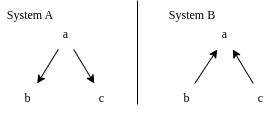
\includegraphics[scale=0.8]{images/lecture1/CR.png}
    \caption{Examples of abstract reduction systems}
\end{figure}


\begin{definition}
    An abstract reduction system $( A, \xrightarrow[A]{} )$ is said to be \textbf{Confluent} if $$\forall a, b, c \in A, \quad a \xrightarrow[A]{*} b \text{ and }  a \xrightarrow[A]{*} c \implies b \downarrow_A c$$
\end{definition}

\begin{definition}
    An abstract reduction system $( A, \xrightarrow[A]{} )$ is said to be \textbf{Semi-confluent} if $$\forall a, b, c \in A, \quad a \xrightarrow[A]{} b \text{ and }  a \xrightarrow[A]{*} c \implies b \downarrow_A c$$
\end{definition}

\begin{theorem}
    For an abstract reduction system, \textbf{Church-Rosser, Confluence and Semi-confluence are equivalent}.
\end{theorem}

\textbf{Proof:} We will prove this theorem in the following three stages. Clearly, the three of them combined result in the theorem stated above.
\begin{enumerate}
    \item $\text{Church-Rosser} \implies \text{Confluence}$
    \item $\text{Confluence} \implies \text{Semi-confluence}$
    \item $\text{Semi-confluence} \implies \text{Church-Rosser}$
\end{enumerate}

First, we will prove that \textbf{if a system is Church-Rosser, it is confluent}. Let $(A, \xrightarrow[A]{})$ be an abstract reduction system that is Church-Rosser. \\
Let $a, b, c \in A : a \xrightarrow[A]{*} b \text{ and } a \xrightarrow[A]{*} c$ \\
By definition, $b \xleftrightarrow[A]{*} c$ \\
Since A is Church-Rosser, $b \xleftrightarrow[A]{*} c \implies b \downarrow_A c$ \\
i.e. $ a \xrightarrow[A]{*} b \text{ and } a \xrightarrow[A]{*} c \implies b \downarrow_A c$, proving that A is confluent


Next, we will prove that \textbf{if a system is Confluent, it is also semi-confluent}. Let $(A, \xrightarrow[A]{})$ be a confluent abstract reduction system. \\
Let $a, b, c \in A : a \xrightarrow[A]{} b \text{ and } a \xrightarrow[A]{*} c$ \\
Since $A \subseteq A^*$, $a \xrightarrow[A]{} b \implies a \xrightarrow[A]{*} b$ \\
Since A is confluent, $a \xrightarrow[A]{*} b \text{ and } a \xrightarrow[A]{*} c \implies b \downarrow_A c$ \\
i.e. $ a \xrightarrow[A]{} b \text{ and } a \xrightarrow[A]{*} c \implies b \downarrow_A c$, proving that A is semi-confluent

Finally, we will prove that \textbf{if a system is semi-confluent, it is also Church-Rosser}. Let $(A, \xrightarrow[A]{})$ be a semi-confluent abstract reduction system. \\
Let $a, b \in A : a \xleftrightarrow[A]{*} b$ \\
Let $p$ be the shortest path connecting $a$ and $b$ in $A^{\leftrightarrow ^*}$. We will use induction on $|p|$ to prove that $a$ and $b$ are joinable. \\
\textbf{Base case:} For $p=0$, we have $a=b$ which makes them trivially joinable. \\
\textbf{Induction step:} Let it be true that if the shortest path connecting $a$ and $b$ in $A^{\leftrightarrow ^*}$ is $|p|$, then $a$ and $b$ are joinable in $A$. We will prove that this is also true for $|p|+1$.

Let $a, b' \in A$ such that the shortest path connecting them in $A^{\leftrightarrow ^*}$ is of length $|p|+1$. Then, $\exists b \in A :$ the shortest path connecting $a$ and $b$ in $A^{\leftrightarrow ^*}$ is $|p|$ and $b \xleftrightarrow[A]{} b'$. Since our induction hypothesis holds true for $|p|$, $a$ and $b$ are joinable (they both reduce to some $c \in A$).


\begin{figure}[htbp]
    \center
    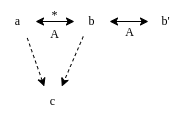
\includegraphics[scale=0.8]{images/lecture1/induction1.png}
    \caption{Abstract reduction system representing the induction step}
\end{figure}
We now have 2 cases. 

\textbf{Case 1:} $b \xleftarrow[A]{} b'$ 

\begin{figure}[htbp]
    \center
    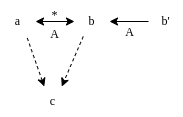
\includegraphics[scale=0.8]{images/lecture1/induction2.png}
    \caption{Abstract reduction system in case 1}
\end{figure}
$b' \xrightarrow[A]{} b \xrightarrow[A]{*} c$. Therefore, $a \downarrow _A b'$. 

\textbf{Case 2:} $b \xrightarrow[A]{} b'$

\begin{figure}[htbp]
    \center
    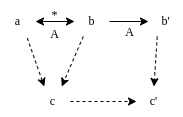
\includegraphics[scale=0.8]{images/lecture1/induction3.png}
    \caption{Abstract reduction system in case 2}
\end{figure}
Here we have $b \xrightarrow[A]{} b'$ and $b \xleftrightarrow[A]{*} c$. Since $A$ is semi-conflient, $b'$ and $c$ must be joinable. That is, $\exists c' \in A : b' \xrightarrow[A]{*} c' \text{ and } c \xrightarrow[A]{*} c'$.  Since $a \xrightarrow[A]{*} c \xrightarrow[A]{*} c'$, we have $a \xrightarrow[A]{*} c'$. Hence, $a \downarrow _A b'$


In either case, we have shown that $a \downarrow _A b'$, which completes our induction. We have proven that $a \xleftrightarrow[A]{*} b \implies a \downarrow_A b$, which means A is also Church-Rosser.

This completes our proof that Church-Rosser, Confluence and Semi-confluence are equivalent properties of an abstract reduction system. While it may seem redundant to have multiple terms to refer to the same thing, they each give us a different perspective of looking at the same property which can prove to be helpful.


\subsection{Address space}
Data structures provide a way to organize and address data. For a data structure, a valid set of addresses form its address space. This is \textbf{not} a formal definition of address spaces and is only meant to give a broad idea. We will look at an example below to illustrate one way of addressing a binary tree. Let us consider the following addressing of a binary tree: each edge is labelled $1$ or $2$ depending on whether it leads to the left or right descendant of a node; the address of each node is obrained by appending the label of the edge leading into it to the address of its parent, with the root being $\epsilon$. Look at the figure below to bettter understand this.
\begin{figure}[htbp]
    \center
    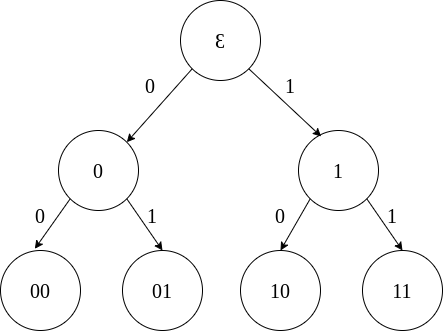
\includegraphics[scale=0.4]{images/lecture1/address.png}
    \caption{Addressing a binary tree}
\end{figure}

The address space for this binary tree would be the set $S = \{\epsilon, 0, 00, 01, 1, 10, 11 \}$. The set $S_1 = \{ \epsilon, 0, 00, 01, 1 \}$ would also be a valid address space for some binary tree but the set $S_2 = \{ 0, 00, 1 \}$ would not, since it does not contain $\epsilon$, the address of the root.

\newpage
\section{Lecture 5}

\subsection{Terms}

\paragraph{ARS} Abstract Reduction System

\paragraph{Terminating ARS} An ARS is terminating \emph{iff.} it has no infinite runs.

\subsection{Well Founded Induction(WFI)}

This is property of an abstract reduction system. A system having this property implies that,

$$
\forall x \in A. \left( \forall y \in A. \ x \successor y \implies P(y) \right) \implies P(x)
$$

in other words,
$P(x)$ is satisfied if $\forall y. x \successor y \implies P(y)$ is satisfied.

\begin{theorem}
    Let, $(A, \longrightarrow)$ be an ARS, then $A$ satisfies WFI iff. $(A, \longrightarrow)$ is terminating.
\end{theorem}

\begin{proof}
    \text{} \\
    \textbf{1. If $\longrightarrow$ terminates, then $A$ satisfies WFI.} \\
    \emph{Proof by contraposition.} Assume that WFI does not hold. \\
    That implies that $\neg P(a_0)$ for some $a_0 \in A$. Since we assumed that WFI does not hold, $\exists a_1$, such that, $a_0 \successor a_1$ and $\neg P(a_1)$. Using the same arguement, $\exists a_2$, such that, $a_1 \successor a_2$ and $\neg P(a_2)$. Hence there is an infinite chain $a_0 \successor a_1 \successor a_2 \successor ...$, i.e. $\longrightarrow$ does not terminate. \\
    \\
    \textbf{2. If $A$ satisfies WFI, then $\longrightarrow$ terminates.} \\
    \emph{Proof by WFI.} Let,
    $$
    P(x) := \text{there is no infinite chain starting from x}.
    $$
    Clearly, if there is no infinite chain starting from any successor of $x$, then there is no infinite chain starting from $x$. Hence, WFI holds and we can conclude that $P(x)$ holds for all $x$, i.e., $\longrightarrow$ terminates.
\end{proof}

\subsection{Confluence}

Order of evaluation does not matter.

\paragraph{Joinable} $x$ and $y$ are joinable, denoted by $\downarrow$ \emph{iff.} they have the same normal form.

\paragraph{Local Confluence} An element $x \in A$ is said to be locally confluent if $\forall y, z \in A, z \lsuccessor x \successor y$ $\exists w : y \too w \ltoo z$, in other words, $y \downarrow z$.

\paragraph{\rightarrow} If a system is terminating and has local confluence for all vertices, then the system has \textbf{confluence}.

\subsection{Interative Evaluation}

\textbf{TODO}


\end{document}
